\documentclass[10pt]{article}
\setlength{\parskip}{0.25\baselineskip}
\usepackage[margin=1in]{geometry} 
\usepackage{amsmath,amsthm,amssymb, graphicx, multicol, array}
\usepackage[font=small,labelfont=bf]{caption}
\usepackage{float}
\usepackage{bbm}

\newcommand{\supp}{{\text{supp}}} 
\newcommand{\bv}{{\text{BV}}}
\newcommand{\ac}{{\text{AC}}}
\newcommand{\vol}{{\text{Vol}}}

\newenvironment{problem}[2][]{\begin{trivlist}
\item[\hskip \labelsep {\bfseries #1}\hskip \labelsep {\bfseries #2.}]}{\end{trivlist}}

\begin{document}
 
\title{Homework \#6}
\author{Eric Tao\\
Math 123: Homework \#6}
\maketitle

\begin{problem}{Question 1}

Let $L = D - W$ be the unnormalized graph Laplacian associated to a graph $\mathcal{G} = (V,W)$ on points $V = \{ x_i \}_{i=1}^n$ with symmetric weight matrix $W$ and diagonal degree matrix $D$. Let $\{ C, \overline{C} \}$ be any partition of $V$, and let:

$$ f^C_i = \begin{cases} -\sqrt{\vol(\overline{C})/\vol(C)} & \text{ if } x_i \in C \\ \sqrt{\vol(C)/\vol(\overline{C})} & \text{ if } x_i \in \overline{C} \end{cases} $$

(a) Prove that $\langle Df^C, \mathbbm{1} \rangle = 0$.

(b) Prove that $(f^C)^T D f^C = \vol(V)$.

(c) Prove that $(f^C)^T L f^C = \vol(V) \cdot \text{Ncut}(C, \overline{C})$.

\end{problem}

\begin{proof}[Solution]

(a)

We notice, that this amounts to summing up the components of $Df^C$. First, consider some $x_i$ such that $x_i \in C$. Then, we have that, with the notation $W(x_i, x_j) = w_{ij}$:

$$(Df^C)_i = \sum_{x_j \in \mathcal{G}}  W(x_i, x_j) \cdot -\sqrt{\vol(\overline{C})/\vol(C)} $$

Summing over $x_i \in C$, we find that:

$$ \sum_{x_i \in C} (Df^C)_i =  \sum_{x_i \in C}  \sum_{x_j \in \mathcal{G}}  W(x_i, x_j) \cdot -\sqrt{\vol(\overline{C})/\vol(C)}$$

Here, we notice though, that, by definition, the double summation is exactly equal to $\vol(C)$! Thus, we have that:

$$ \sum_{x_i \in C} (Df^C)_i = - \vol(C) \cdot \sqrt{\vol(\overline{C})/\vol(C)} = - (\vol(C) \vol(\overline{C}))^{1/2} $$

It is not hard to see that for $x_i \in \overline{C}$, that we get a similar result:

$$ \sum_{x_i \in \overline{C}} (Df^C)_i = \vol(\overline{C}) \cdot \sqrt{\vol(C)/\vol(\overline{C})} =  (\vol(C) \vol(\overline{C}))^{1/2}$$

Thus, summing over all $x_i$ in $(Df^C)_i$, we find that:

$$\sum_{x_i \in \mathcal{G}} (Df^C)_i =  \sum_{x_i \in C} (Df^C)_i +  \sum_{x_i \in \overline{C}} (Df^C)_i =  - (\vol(C) \vol(\overline{C}))^{1/2} +  (\vol(C) \vol(\overline{C}))^{1/2} = 0$$

as desired.

(b)

In a similar fashion to (a), we will look at this term by term. We already found that, for $x_i \in C$, that $(Df^C)_i = \sum_{x_j \in \mathcal{G}}  W(x_i, x_j) \cdot -\sqrt{\vol(\overline{C})/\vol(C)} $. Then, we have that in the inner product with $(f^C)^T$, the component that corresponds to this component will multiply to find:

$$  -\sqrt{\vol(\overline{C})/\vol(C)} \cdot \left( \sum_{x_j \in \mathcal{G}}  W(x_i, x_j) \cdot -\sqrt{\vol(\overline{C})/\vol(C)} \right) = \frac{\vol(\overline{C})}{\vol(C)} \cdot \sum_{x_j \in \mathcal{G}}  W(x_i, x_j) $$

Then, summing over the $x_i \in C$, we find that:

$$ \sum_{x_i \in C} \frac{\vol(\overline{C})}{\vol(C)} \cdot \sum_{x_j \in \mathcal{G}}  W(x_i, x_j) =  \frac{\vol(\overline{C})}{\vol(C)} \sum_{x_i \in C} \sum_{x_j \in \mathcal{G}} W(x_i, x_j) = \frac{\vol(\overline{C})}{\vol(C)} \vol(C) = \vol(\overline{C})$$

Without writing it out, it should be clear that in the same way, if $x_i \in \overline{C}$, then summing over those, we retrieve $\vol{C}$.

Thus, we have that:

$$ (f^C)^T D f^C = \sum_{x_i \in C}\left(  \frac{\vol(\overline{C})}{\vol(C)} \cdot \sum_{x_j \in \mathcal{G}}  W(x_i, x_j) \right) +  \sum_{x_i \in \overline{C}} \left( \frac{\vol(C)}{\vol(\overline{C})} \cdot \sum_{x_j \in \mathcal{G}}  W(x_i, x_j)\right) = \vol(\overline{C}) + \vol(C) =$$
$$ \sum_{x_i \in \overline{C}, x_j \in \mathcal{G}} W(x_i, x_j) + \sum_{x_i \in C, x_j \in \mathcal{G}} W(x_i, x_j) = \sum_{x_i, x_j \in \mathcal{G}} W(x_i, x_j) = \vol(G)$$

(c)

We recall from homework 5, question 2, we found that for any vector $y$, that $y^T L y = \frac{1}{2} \sum_i \sum_j w_{ij} (y_i - y_j)^2$. Applying this for $y = f^C$, we have that:

$$ (f^C)^T L f^C = \frac{1}{2}  \sum_i \sum_j w_{ij} ((f^C)_i - (f^C)_j)^2$$

Clearly, if $i = j$, this value is 0. Further, if $x_i, x_j \in C$, or if $x_i, x_j \in \overline{C}$, then of course we have that $(f^C)_i  =  (f^C)_j$, and thus disappears. Lastly, we notice that this double counts everything, and that under interchange of $x_i, x_j$, the value is unchanged due to for $x_i \in C, x_j \in \overline{C}$, $ ((f^C)_i - (f^C)_j)^2 =  ((f^C)_j - (f^C)_i)^2$. So, we can say that:

$$(f^C)^T L f^C = \frac{1}{2}  \sum_i \sum_j w_{ij} ((f^C)_i - (f^C)_j)^2 = \sum_{x_i \in C, x_j \in \overline{C}} w_{ij} \left(\sqrt{\frac{\vol(\overline{C})}{\vol(C)}}+ \sqrt{\frac{\vol(C)}{\vol(\overline{C})}}\right)^2 =$$

$$  \sum_{x_i \in C, x_j \in \overline{C}} w_{ij} \left( \frac{\vol(\overline{C})+ \vol(C)}{\sqrt{\vol(C)\vol(\overline{C})}} \right)^2 = \sum_{x_i \in C, x_j \in \overline{C}} w_{ij}\vol(G) \frac{\vol(\overline{C})+ \vol(C)}{\vol(C)\vol(\overline{C})}=$$ 
$$\vol(G) \sum_{x_i \in C, x_j \in \overline{C}}w_{ij} \left( \frac{1}{\vol(C)} + \frac{1}{\vol(\overline{C})} \right) = \vol(G) \cdot \text{Ncut}(C,\overline{C}) $$

as desired.

\end{proof}

\begin{problem}{Question 2}

Recall that one construction of the weight matrix for a graph on data points $\{ x_i \}_{i=1}^n$ is to use the Gaussian kernel 

$$W_{ij} = \begin{cases} \exp(-\Vert x_i - x_j \Vert_2^2/\sigma^2) &  i \not = j \\ 0 & i = j \end{cases}$$

for some choice of $\sigma > 0$.

(a) What happens to the resulting Laplacian matrix as $\sigma \to 0$?

(b) What happens to the resulting Laplacian matrix as $\sigma \to \infty$?

\end{problem}

\begin{proof}[Solution]

(a)

Qualitatively, we notice that as $\sigma \to 0$, then this amounts to narrowing the Gaussian, and making it sharper around $\Vert x_i - x_j \Vert_2^2 = 0$. We can imagine in the limiting case that it has the same effect as the Dirac measure, where we assign the value to be 1 if and only if the values are the same. In such a limiting case, we would see that the Laplacian matrix would converge towards a matrix of all 0s (assuming each data point takes on distinct values), as we may pick a $\sigma$ such that $\Vert x_i - x_j \Vert_2^2 < \epsilon$.

Formally: Let $\epsilon > 0$ be given. Since we know that as $t \to \infty, e^{-t} \to 0$, we can choose $\delta$ such that so long as $t > \delta$, $e^{-t} < \epsilon$.

WLOG, choose $x_i = 0$, and fix some $x_j$ such that $x_j \not = x_i$.Of course the sequence $\Vert x_j \Vert_2^2 n \to \infty$ for $n \in \mathbb{N}, n \to \infty$. Thus, we may choose $N \in \mathbb{N}$ such that for all $m > N$, $\Vert x_j \Vert_2^2 m > \delta$. Further, since we know that as $x \to 0, 1/x \to \infty$, we may choose $L$ such that for all $l > L$, $1/l > m$.

Choose $\sigma$ such that  $\sigma > L+1$. Then, we have that:

$$ \frac{\Vert x_j \Vert_2^2}{\sigma^2} > \frac{\Vert x_j \Vert_2^2}{(L+1)^2} > \Vert x_j \Vert_2^2 m > \delta$$

Thus, we have that for this choice of $\sigma$, $e^{-\Vert x_j \Vert_2^2/\sigma^2} < \epsilon$. Since this can be done for any $x_i \not = x_j$, we have that these weights go to 0 for all distinct points.

We can then conclude that all edges between distinct points go to a weight of 0, which implies that, assuming our points are distinct, and that we do not consider any edges from $x_i \to x_i$, that is, any loops, that $L$ converges to the 0 matrix.

(b)

In the opposite case, where we take $\sigma \to \infty$, we expect instead for edge weights to converge to the value 1. WLOG, choose $x_i = 0$, and fix some $x_j$. Let $\epsilon > 0$ be given. Since the exponential is continuous, there exists $\delta > 0$ such that $ \Vert 1  - e^{t} \Vert < \epsilon$ for all $|t| < \delta$.

Now, by the Archimidean principle, there exists an $N \in \mathbb{N}$ such that $\frac{\Vert x_j\Vert_2^2 }{N} < \delta$. Consider $\sigma > N$. Then, we have that:

$$ \frac{\Vert x_j \Vert_2^2}{\sigma^2}\leq  \frac{\Vert x_j \Vert_2^2}{N^2} <  \frac{\Vert x_j \Vert_2^2}{N} < \delta$$

Thus, for any $\sigma > N$, we have that $\Vert 1 - e^{\Vert x_j \Vert_2^2/\sigma^2} \Vert < \epsilon$, and we are done. Since this can be done for all $x_i, x_j$ in the limit, this works for every point in our data set, where we're not concerned about issues on the supremum being equal to $\infty$, since we are in the limiting cases.

Thus, in terms of the Laplacian matrix, we expect things to converge to $n$ on the diagonal, and $-1$ on every other entry, where $n$ is the dimensionality of the Laplacian, or, equivalently, the number of data points.



\end{proof}

\begin{problem}{Question 3}

Load the dataset "SalinasA\_corrected.mat" and "Salinas-S-groundtruth".

(a) Run spectral clustering on this data, using a sparse Laplacian with different numbers of nearest neighbors and $K = 6$ clusters. How do the results compare to the ground truth data?

(b) Plot the first 10 eigenvalues of the data for different choices of $\sigma$. What does the eigengap estimate as the number of cluster for these choices of $\sigma$?

(c) Compare the projections onto the first three principal components with the first three Laplacian eigenvectors by plotting both sets in different figures using 'scatter3'. How do the representations differ qualitatively?


\end{problem}

\begin{proof}[Solution]

Here follows some spectral clustering on this data, with a sparse Laplacian, 6 clusters, and various numbers of nearest neighbors, with a fixed value of $\sigma = 10000$:

\begin{figure}[H]
\centering
\begin{minipage}{.5\textwidth}
  \centering
  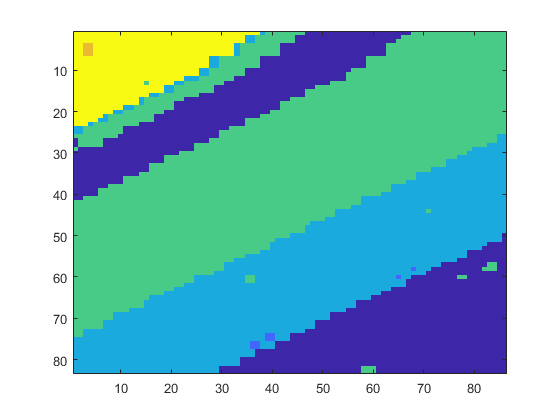
\includegraphics[width=\linewidth]{5_nn}
  \captionof{figure}{10 Nearest Neighbors}
  \label{fig:test1}
\end{minipage}%
\begin{minipage}{.5\textwidth}
  \centering
  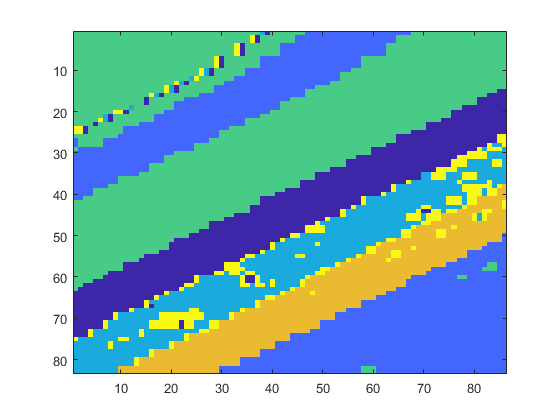
\includegraphics[width=\linewidth]{10_nn}
  \captionof{figure}{50 Nearest Neighbors}
  \label{fig:test2}
\end{minipage}
\end{figure}

\begin{figure}[H]
\centering
\begin{minipage}{.5\textwidth}
  \centering
  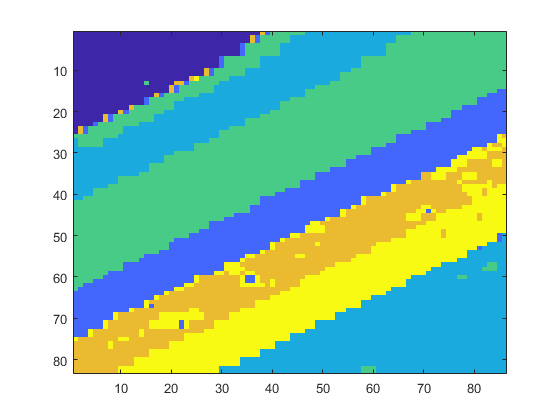
\includegraphics[width=\linewidth]{50_nn}
  \captionof{figure}{100 Nearest Neighbors}
  \label{fig:test1}
\end{minipage}%
\begin{minipage}{.5\textwidth}
  \centering
  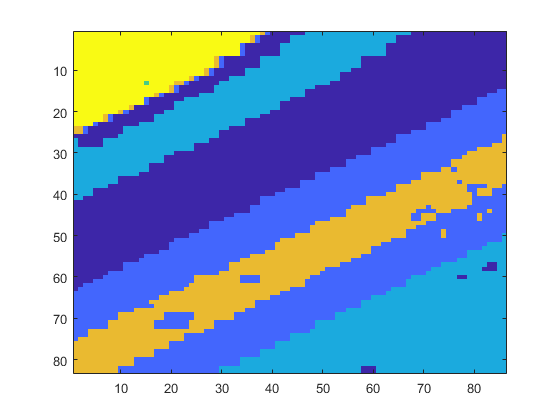
\includegraphics[width=\linewidth]{100_nn}
  \captionof{figure}{500 Nearest Neighbors}
  \label{fig:test2}
\end{minipage}
\end{figure}

In comparison, this is the groundtruth:

\begin{center}
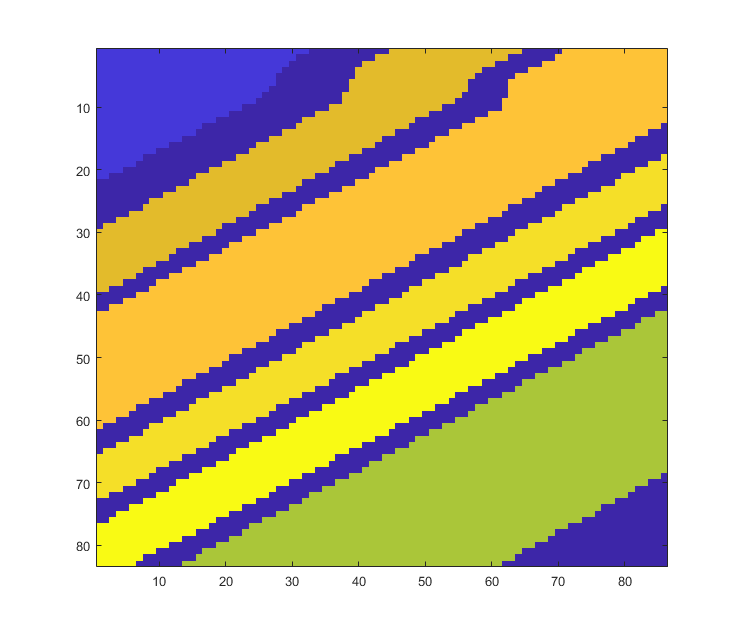
\includegraphics[width=\linewidth]{ground_truth}
\captionof{figure}{Salinas A Groundtruth}
\end{center}

We can see the structures pretty easily, and qualitatively, we have a decent match. There is definitely some tuning that could be done here, the boundary can be messy, and perhaps we need better separation of points with a higher $\sigma$ value.

(b)

Here follows the first 10 eigenvalues for specific choices of $\sigma$, and a fixed $500$ nearest neighbors:

\begin{figure}[H]
\centering
\begin{minipage}{.5\textwidth}
  \centering
  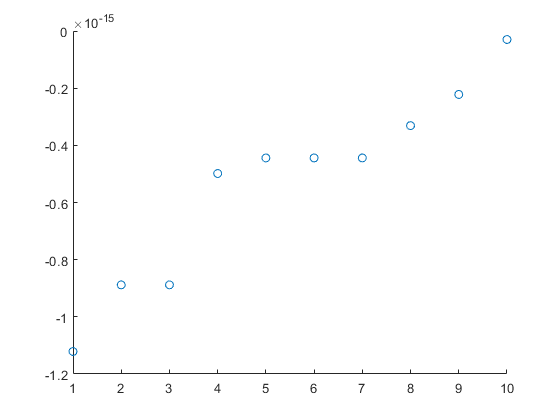
\includegraphics[width=\linewidth]{1_sigma}
  \captionof{figure}{$\sigma=1$}
  \label{fig:test1}
\end{minipage}%
\begin{minipage}{.5\textwidth}
  \centering
  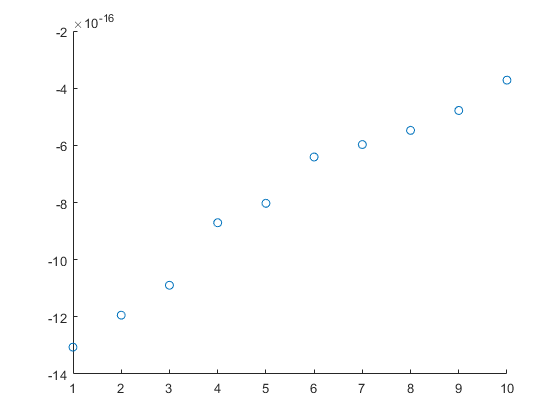
\includegraphics[width=\linewidth]{100_sigma}
  \captionof{figure}{$\sigma=100$}
  \label{fig:test2}
\end{minipage}
\end{figure}

\begin{figure}[H]
\centering
\begin{minipage}{.5\textwidth}
  \centering
  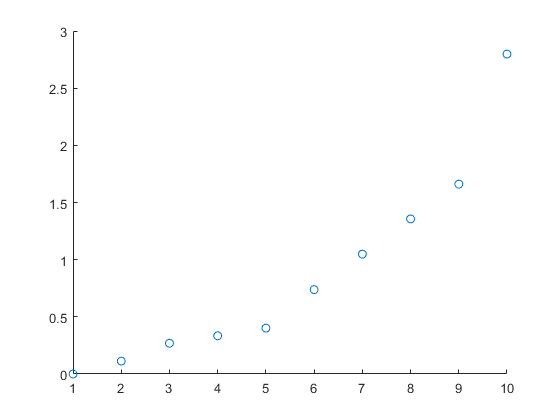
\includegraphics[width=\linewidth]{10000_sigma}
  \captionof{figure}{$\sigma=10000$}
  \label{fig:test1}
\end{minipage}%
\begin{minipage}{.5\textwidth}
  \centering
  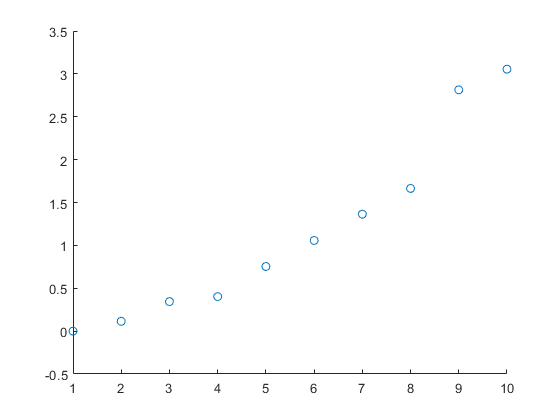
\includegraphics[width=\linewidth]{1000000_sigma}
  \captionof{figure}{$\sigma=1000000$}
  \label{fig:test2}
\end{minipage}
\end{figure}

At the scale of $\sigma =1, 100$, the values are close to float rounding errors so probably should be discarded, but they seem to suggest $3$ clusters, looking at the jump from the 3rd to the 4th eigenvalue.

At the scale of $\sigma = 10000, 1000000$, we see a clear jump at $9 \to 10$ for 10k, and $8 \to 9$ for $\sigma = 1000000$. This seems to suggest that as we increase $\sigma$, we get more separation in the data, and thus more reasonable distinct clustering.

(c)

Here, we compare projection onto the Laplacian eigenvectors for 100 nearest neighbors, $\sigma = 10000$, and PCA:

\begin{figure}[H]
\centering
\begin{minipage}{.5\textwidth}
  \centering
  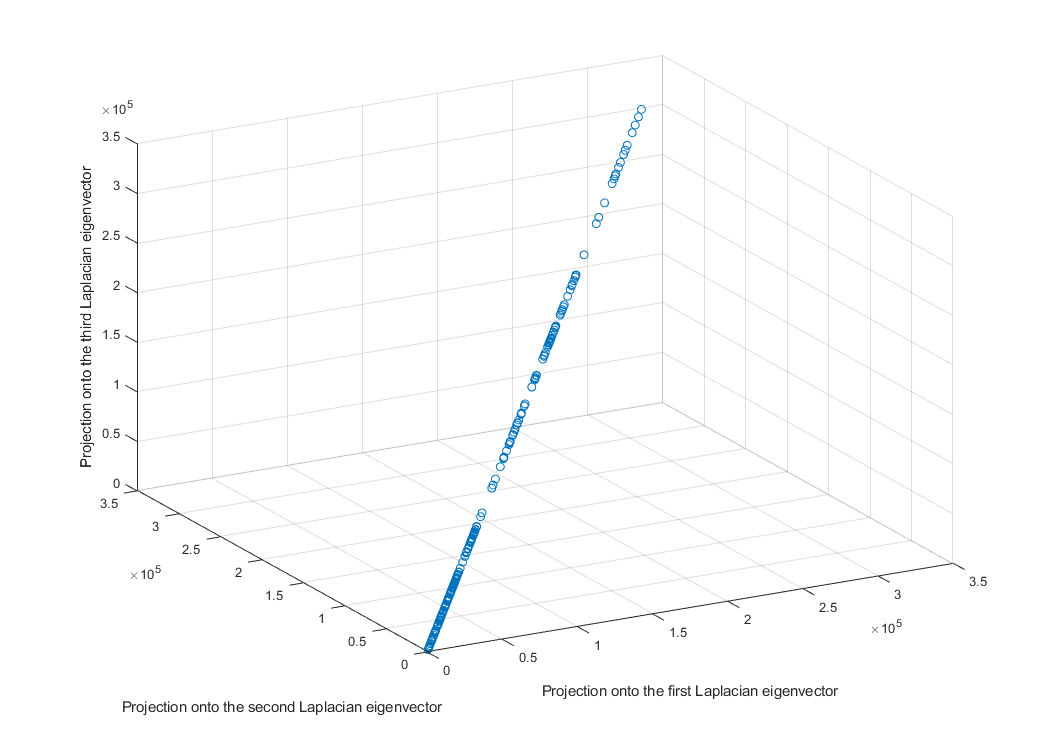
\includegraphics[width=\linewidth]{laplacian_projection}
  \captionof{figure}{Projection onto the 3 Laplacian eigenvectors with smallest eigenvalues}
  \label{fig:test1}
\end{minipage}%
\begin{minipage}{.5\textwidth}
  \centering
  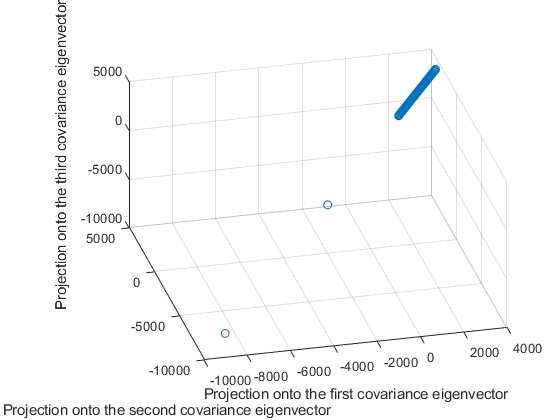
\includegraphics[width=\linewidth]{covariance_projection}
  \captionof{figure}{Projection onto the 3 principal components of largest variance}
  \label{fig:test2}
\end{minipage}
\end{figure}

Qualitatively, we notice that the Laplacian projections are strictly positive, whereas the projections onto the eigenvalues of the covariance matrix can take on both positive or negative values. Structurally, they seem to be very similar, but it is fairly hard to tell.


\end{proof}



\end{document}